\documentclass[border=15pt]{standalone}
\usepackage{amsmath, amssymb}
\usepackage{tikz}
\usetikzlibrary{arrows.meta}

\definecolor{block0}{HTML}{E53935}
\definecolor{block1}{HTML}{1E88E5}
\definecolor{block2}{HTML}{43A047}
\definecolor{block3}{HTML}{FB8C00}

\begin{document}
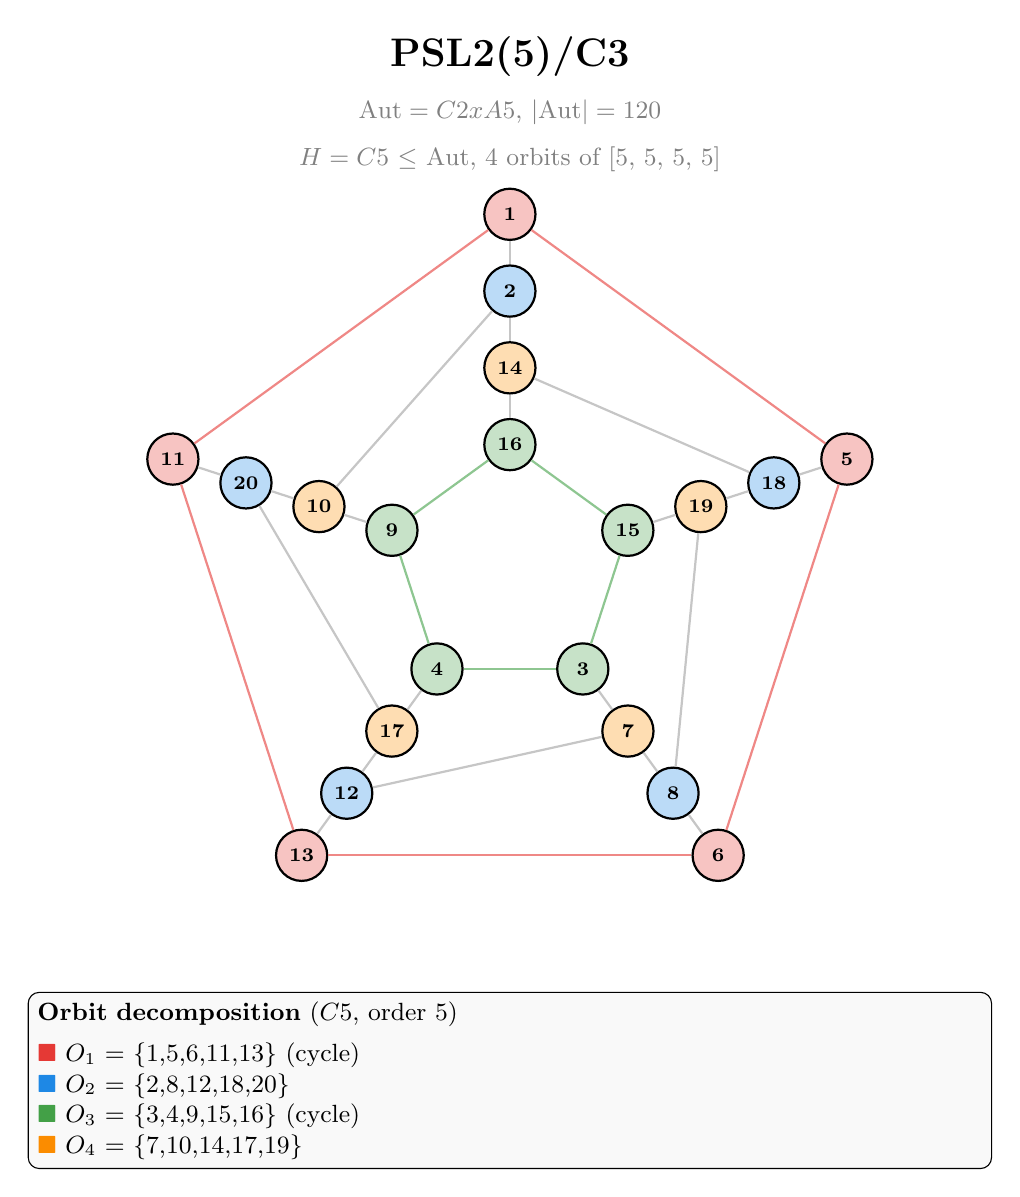
\begin{tikzpicture}[
  vertex/.style={circle, draw, thick, minimum size=6.5mm, inner sep=0pt,
                 font=\scriptsize\bfseries},
  edge/.style={thick, gray!45},
  title/.style={font=\Large\bfseries},
  subtitle/.style={font=\small, text=gray},
]

\node[title] at (0, 6.5) {PSL2(5)/C3};
\node[subtitle] at (0, 5.8) {$\mathrm{Aut} = C2 x A5$, $|\mathrm{Aut}| = 120$};
\node[subtitle] at (0, 5.2) {$H = C5$ $\leq$ $\mathrm{Aut}$, 4 orbits of [5, 5, 5, 5]};

\node[vertex, fill=block0!30] (v1) at (0.000, 4.500) {1};
\node[vertex, fill=block1!30] (v2) at (0.000, 3.525) {2};
\node[vertex, fill=block2!30] (v3) at (0.926, -1.274) {3};
\node[vertex, fill=block2!30] (v4) at (-0.926, -1.274) {4};
\node[vertex, fill=block0!30] (v5) at (4.280, 1.391) {5};
\node[vertex, fill=block0!30] (v6) at (2.645, -3.641) {6};
\node[vertex, fill=block3!30] (v7) at (1.499, -2.063) {7};
\node[vertex, fill=block1!30] (v8) at (2.072, -2.852) {8};
\node[vertex, fill=block2!30] (v9) at (-1.498, 0.487) {9};
\node[vertex, fill=block3!30] (v10) at (-2.425, 0.788) {10};
\node[vertex, fill=block0!30] (v11) at (-4.280, 1.391) {11};
\node[vertex, fill=block1!30] (v12) at (-2.072, -2.852) {12};
\node[vertex, fill=block0!30] (v13) at (-2.645, -3.641) {13};
\node[vertex, fill=block3!30] (v14) at (0.000, 2.550) {14};
\node[vertex, fill=block2!30] (v15) at (1.498, 0.487) {15};
\node[vertex, fill=block2!30] (v16) at (0.000, 1.575) {16};
\node[vertex, fill=block3!30] (v17) at (-1.499, -2.063) {17};
\node[vertex, fill=block1!30] (v18) at (3.352, 1.089) {18};
\node[vertex, fill=block3!30] (v19) at (2.425, 0.788) {19};
\node[vertex, fill=block1!30] (v20) at (-3.352, 1.089) {20};

\draw[edge] (v1) -- (v2);
\draw[thick, block0!60] (v1) -- (v5);
\draw[thick, block0!60] (v1) -- (v11);
\draw[edge] (v2) -- (v10);
\draw[edge] (v2) -- (v14);
\draw[thick, block2!60] (v3) -- (v4);
\draw[edge] (v3) -- (v7);
\draw[thick, block2!60] (v3) -- (v15);
\draw[thick, block2!60] (v4) -- (v9);
\draw[edge] (v4) -- (v17);
\draw[thick, block0!60] (v5) -- (v6);
\draw[edge] (v5) -- (v18);
\draw[edge] (v6) -- (v8);
\draw[thick, block0!60] (v6) -- (v13);
\draw[edge] (v7) -- (v8);
\draw[edge] (v7) -- (v12);
\draw[edge] (v8) -- (v19);
\draw[edge] (v9) -- (v10);
\draw[thick, block2!60] (v9) -- (v16);
\draw[edge] (v10) -- (v20);
\draw[thick, block0!60] (v11) -- (v13);
\draw[edge] (v11) -- (v20);
\draw[edge] (v12) -- (v13);
\draw[edge] (v12) -- (v17);
\draw[edge] (v14) -- (v16);
\draw[edge] (v14) -- (v18);
\draw[thick, block2!60] (v15) -- (v16);
\draw[edge] (v15) -- (v19);
\draw[edge] (v17) -- (v20);
\draw[edge] (v18) -- (v19);

\node[draw, rounded corners, fill=gray!5, text width=12cm, align=left, font=\small]
  at (0, -6.5) {
  \textbf{Orbit decomposition} ($C5$, order 5) \\[4pt]
  \textcolor{block0}{$\blacksquare$} $O_{1}$ = \{1,5,6,11,13\} (cycle) \\
  \textcolor{block1}{$\blacksquare$} $O_{2}$ = \{2,8,12,18,20\} \\
  \textcolor{block2}{$\blacksquare$} $O_{3}$ = \{3,4,9,15,16\} (cycle) \\
  \textcolor{block3}{$\blacksquare$} $O_{4}$ = \{7,10,14,17,19\}
};

\end{tikzpicture}
\end{document}